\documentclass[11pt, a4paper]{report}
\usepackage[utf8]{inputenc}
\usepackage{float}
\usepackage{array}
\usepackage{amsmath}
\usepackage{amssymb}
\usepackage{amsfonts}
\usepackage{latexsym}
\usepackage{graphicx}
\usepackage{tabularx}
\usepackage{ltxtable}
\usepackage{longtable}
\usepackage{color, colortbl}
\usepackage{caption}%\usepackage{subcaption}
\usepackage{ifpdf}
\usepackage[hidelinks]{hyperref}
\usepackage{url}
\usepackage{xtab}
\usepackage[hmargin=3cm,vmargin=3cm]{geometry}
\usepackage[norsk]{babel}
\usepackage[parfill]{parskip}
\usepackage{pdfpages}
\usepackage{listings}
\usepackage{subfigure}
\usepackage{xcolor,colortbl}

% Begin chapter numbering
\usepackage[T1]{fontenc}
\usepackage{titlesec, blindtext, color}

\definecolor{gray75}{gray}{0.75}
\newcommand{\hsp}{\hspace{20pt}}
\titleformat{\chapter}[hang]{\Huge\bfseries}{\thechapter\hsp\textcolor{gray75}{|}\hsp}{0pt}{\Huge\bfseries}
% End chapter numbering

% Add numbering to subsubsection
\setcounter{secnumdepth}{3}
\setcounter{tocdepth}{3}

\definecolor{Gray}{gray}{0.9}

% Header packages
\usepackage{fancyhdr}
\pagestyle{fancy}
\rhead{Chapter: \thechapter}

% Custom 
%\newcommand{\newCommandName}{text to insert} % Defines a variable in LaTeX
\newcommand{\comment}[1]{} \comment{This is a block comment wrapped in curly brackets}
%\renewcommand{\thefootnote}{\roman{footnote}}

\begin{document}
%\pagecolor{yellow!30} % Uncomment for debugging floats
\pagenumbering{gobble}


\begin{titlepage}
\begin{center}
\vspace*{1in}
{\LARGE Eksperter i Team}
\par
\vspace{1cm}


\begin{figure}[ht!]
\centering
%
\includegraphics[width=25mm]{images/logo.png}
%\caption{A simple caption}
\label{overflow}
\end{figure}


{\LARGE Stereo}
\par
\vspace{0.6in}
{\LARGE Project report}
\par
\vspace{0.2in}
{\Large Group 1}
\par
\vfill
\par
\vspace{0.5in}
Our names\\ \ldots here\\
\par
\vspace{0.4cm}
\today
\end{center}
\end{titlepage}

%\newpage
%
%\input{section/abstract}

\tableofcontents
\newpage
\pagenumbering{arabic}

%%%
% Put new includes here
%%%

\chapter{Introduksjon}
\section{Gruppen} 
\subsection{Emil Bjørlykhaug}
Går undervannsteknologi, 2-årig master. Har tidligere gått Automasjon ved Hials.
Som folk flest hadde jeg hørt en del snakk om EiT på forehand, noe positivt, noe negativt. 
Jeg hadde ikke noen store forventninger ang. selve prosjektet vi skulle gjennomføre,
 men hadde en del forventninger til det å jobbe i gruppe, og å lære hvordan gruppedynamikk 
fungerer sett fra både et teoretisk og praktisk perspektiv. Jeg har tidligere selv jobbet 
en del i grupper, men oftest har medlemmene av desse gruppene vært folk jeg har kjent 
fra før. I et tilfelle når jeg studerte på Hials hadde foreleser ansvaret med å dele opp gruppe, 
så jeg havnet på en gruppe med bare ukjente personer. Jeg følte dette er en god måte å 
utfordre folk sosialt, og følte jeg i løpet av semesteret ble utrolig godt kjent med de jeg 
måtte jobbe sammen med.
Jeg er ikke av typen som roper høgest i diskusjoner, og kan ofte bli litt passiv i 
gruppesammenhenger om jeg ikke føler jeg har noe å stille med, men håper 
EiT kan gjøre meg til et bedre gruppemedlem. Jeg er positivt innstilt til faget 
og håper på høgt læringsutbytte.

\subsection{David Hovind} Jeg har ikke hørt så mye om EiT fra før så jeg vet ikke helt hva det går ut på. 
Jeg har derfor et åpent sinn til faget og ser på det som en positiv utfordring. 
Som regel så foretrekker jeg ikke gruppearbeid fordi man blir avhengig av alle andre i gruppen og de blir avhengige av deg. 
Av den grunn så liker jeg best å jobbe selvstendig, siden det finnes mange forskjellige typer mennesker og man vet aldri 
hvilke typer mennesker man havner på gruppe med. Jeg forventer å bli bedre til å kjenne meg selv og få litt innsikt i 
hvordan det er å reflektere over gruppearbeidet.

\subsection{Kristoffer Løvall}
Jeg fikk høre litt forskjellig om Eksperter i Team før dette semesteret, men har 
prøvd å holde de negative holdningene til faget ute. Jeg starter semesteret 
derfor semesteret med en positiv innstilling, spesielt siden landsbyens tema 
virker veldig interessant og spennende. Jeg forventer at det blir lærerikt å 
jobbe på tvers av fagfelt og interesser, og at tverrfagligheten bidrar til å 
designe et godt produkt. På grunn av tidligere gruppearbeid i forhåndsbestemte 
grupper med ukjente personer har jeg ikke store forventninger til det sosiale, 
noe som på sitt vis kan være positivt ettersom det da ikke er mye som skal til 
for at dette går over forventning. Jeg har også jobbet relativt mye i grupper 
gjennom porsjekter både på NTNU og Høgskolen i Bergen, der jeg ofte har endt opp 
med å ta ansvar og fungere som en gruppeleder. Jeg vet også at jeg kan bli noe 
kontrollerede når jeg blir veldig engasjert og brenner for noe.  Målet mitt for 
Eksperter i Team er å "prøve noe nytt" og være litt mer tilbakeholden på denne 
fronten, prøve å jobbe på linje med alle andre uten å "ta over" for noen og 
kontrollere alle detaljer. Jeg vil bli enklere å jobbe i team med og lære meg 
selv å godta andres løsninger og akseptere disse som de beste løsningene, selv om 
min opprinnelige tanke var noe helt annet. Når det gjelder det faglige håper jeg 
alle har høye forventninger både når det gjelder engasjement for å ende opp med 
gode løsninger, samt det å få en god karakter i faget.
\comment{ foreløpig struktur på rapport:
Sammendrag
Innhold
Introduksjon
	Gruppen
	Initiativet
	Problemet
	Ideen
Pre study
	Mekanikk
	Hardware
	Software
Markedsundersøkelse
	generelt
	4 p'er
Løsning
	valg av løsning
	hardware
	software
		GUI
	diskusjon
Konklusjon
Referanseliste
Vedlegg
}
%\input{section/Sammendrag}
%\input{section/Innhold}
\section{Introduksjon}
	%\input{section/Gruppen}
	%\input{section/Initiativet}	
	%\section{Problemet}

Aktuelle nyheter i oppstartsperioden av dette prosjektet rapporterte om en 
hendelse i Kina, hvor et løpsk lastebilhjul traff en mann som hadde parkert på 
veiskulderen, og dyttet ham over autovernet og ned en skrent. Heldigvis pådro 
han seg ingen større skader i ulykken. Vi tok også kontakt med en lastebilsjåfør
 og maskiningeniør, Olav Rogne, for å forhøre oss om relevante problemstillinger 
til EiT. Hendelsen i Kina, samt intervjuet med yrkessjåføren inspirerte til videre
research av problemet, og følgende problemstilling ble formet:

\begin{center}
\emph{``Hvordan automatisere identifikasjon og varsling av løse hjumuttere?''}
\end{center}

Både på verdensbasis og i Norge er såkalt ``hjulmist'' \cite{hjulmist} et økende problem, ikke bare 
på grunn av materielle skader, men også på grunn av risikoen for menneskelige 
skader og dødsfall. Det finnes flere grunner til løsnede hjul, og gjennom undersøkelser 
gjort i flere land har man kommet fram til fire overordnede årsaker:

\begin{itemize}
\item{ Skader på friksjonsoverflaten mellom mutter, bolt, felg og nav fører til sluring og/eller
vibrasjoner som over tid gjør at bolten/mutteren løsner.}
\item { Temperaturendringer som medfører at bolt og mutter krymper eller vokser, noe som 
endrer spenningene og tiltrekkingsmomentet i koblingen.}
\item{ Manglende ettertrekking av hjulmuttere.}
\item{ Utmatting i bolt grunnet for hard tiltrekking over anbefalt tiltrekkingsmoment som igjen 
fører til strekk over materialets flytegrense (plastisk/varig deformasjon).}
\end{itemize}

For å unngå dette problemet ønsker vi å planlegge og utvikle en spesifikasjon for et system som oppdager 
det løsnende hjulet før det separeres fra vogntoget. Vi ønsker å automatisere både identifikasjon
og varsling slik at sikkerheten både for sjåfør og andre blir drastisk bedret, i tillegg til at de materielle
kostnadene blir redusert.

	%\section{Ideen}
Ideen er å utvikle et produkt som rapporterer sanntidsstatus til lastebilsjåføren 
ved løsnede hjulmuttre. Dette innebærer en måling av hjulmuttrenes tilstand på 
hjulbolten, analyse av disse dataene, og rapportering av nødvendige data 
opp til førerhuset slik at de kan visualiseres på et lett forståelig format.

Den første mulige løsningen som ble oppdaget var måling av mutterposisjon ved 
hjelp av strekklapper. Etter konsultasjon med KA ble det klart 
at denne typen avviksregistrering ville egnet seg best for ettermontering, 
men at det allikevel ville bli et dyrt produkt basert på antall nødvendige 
strekklapper pr. hjul. 

Løsningsalternativ nummer to var en vibrasjonssenor i nav eller aksling, som 
rapporterer tilbake dersom det registreres avvik i vibrasjoner fra ett hjul 
kontra de andre hjulene på kjøretøyet. En slik løsning vil kunne bli billigere 
basert på et lavere behov for komponenter.

Feilmeldingen som kommer opp til sjåfør presenteres så enkelt som mulig for å unngå for mange forstyrrende elementer i dashbordet. Samtidig er nøyaktighet en viktig del av representasjonen, slik at sjåføren sparer tid på å kun ettertrekke de nødvendige muttre.
\section{Prestudy}
	\section{Mekanikk}
\comment{\subsection{Reaksjoner i systemet}}

For å utvikle ideer til hvordan problemstillingen kan løses, er det nødvendig å analysere hva som skjer om en hjulmutter løsner. Det har i denne sammenheng blitt brukt en brainstorming-teknikk for å sammen kunne komme fram til så mange av disse reaksjonene som mulig. Vi har identifisert følgende reaksjoner grunnet endring i mutterens tilstramming:

\begin{table}[h]
\caption{Mekaniske og andre reaksjoner i systemet}
\begin{tabular}{|l|l|}
\hline
\textbf{Mekanisk}                   & \textbf{Annet}                                   \\
\hline
Strekk i bolt ved strammet mutter   & Temperaturendring pga friksjonsvarme ved løsning \\
\hline
Kompresjonsendring i mutter         & Vibrasjonsendringer i understell                 \\
\hline
Torsjonsendring                     & Endring i friksjon mellom bakke og hjul          \\
\hline
Trykkendring mellom mutter og flate & ...                                              \\
\hline
\end{tabular}
\end{table}

\subsection{Håndberegninger av strekk og trykk}

Etter å ha intervjuet yrkessjåfør Olav Rogne, valgte vi å bruke dimensjonene han har oppgitt som utregningseksempel. Det ble opplyst om at det var normalt å bruke mutter av typen M33x3.5 som trekkes til med et tiltrekkingsmoment på 700Nm. Man kan utifra dette enkelt regne ut spenninger som oppstår i bolten.

Momentet som tilføres bolten ved tiltrekking deles opp i to komponenter:
\begin{center}
$M_{tiltrekning}=M_{v}+M_{s}$
\end{center}
Der $M_{v}$ er momentet som oppstår pga friksjonskrefter i gjengeflaten, og $M_{s}$ er momentet som oppstår pga krefter mellom mutter og underlaget. Disse kan igjen bli beskrevet slik:
\begin{center}
$M_{v}=F\cdot tan(\varphi +\varepsilon )\cdot r_{m}$
\end{center}
og
\begin{center}
$M_{s}=\mu 'Fr_{m}$
\end{center}
I disse to formlene tar vi i bruk flere fraktorer. $ r_{m}$ er radiusen som friksjonskraften mot underlaget antas å virke på:
\begin{center}
$r_{m}=\frac{N\o kkelvidde+d_{h}}{4}$
\end{center}
$\varphi$ er gjengenes stigningsvinkel:
\begin{center}
$\varphi =\frac{gjengestigning}{\pi \cdot d_{pich}}$
\end{center}
og $\varepsilon$ er friksjonsvinkelen i skråplanet der kreftene i gjengene virker:
\begin{center}
$\varepsilon =tan^{-1}(\frac{\mu}{cos(\alpha )})$
\end{center}
Her er $\alpha$ halve gjengevinkelen og vi har satt friksjonsfaktor i gjengeene til $\mu=0.08$ \cite{FriksjonsfaktorGjenger} %http://www.kamax.com/fileadmin/user_upload/dokumente/pdf/Bolt_and_Screw_Compendium.pdf

Videre kan vi løse dette for kraften:
\begin{center}
$F_{aksiell}=\frac{M_{tiltrekning}}{(tan(\varphi +tan^{-1}(\frac{\mu }{cos(\alpha )}))+\mu')\frac{N+d_{h}}{4}}$
\end{center}
Siden vi også vet at
\begin{center}
$\sigma=\frac{F}{A}$
\end{center}
Kan vi si at trykket mellom mutter og underlag er:
\begin{center}
$p_{trykkflate}=\frac{F_{aksiell}}{A_{trykkflate}}=\frac{F_{aksiell}}{\frac{\pi }{4}(D_{mutterflate}^{2}-D_{hull}^{2})}$
\end{center}
Videre vet vi at flytegrensen er:

\begin{center}
$\sigma _{f}\approx 250 Mpa-350 Mpa$
\end{center}

Ut ifra disse beregningene har vi kommet fram til at det vil være et overtrykk trykk på 116.6 MPa mellom mutter og flaten mutteren trykker på, samt et strekk på 193 Mpa i bolten.

\subsection{FEM-analyse}

Beregningene i forrige avsnitt kan også simuleres med en "finite element method" (FEM) analyse i programvare tilgjengelig ved NTNU som for eksempel NX 9.0 som er brukt i dette tilfellet. Først blir bolten og mutteren modellert etter dimensjonene for en M33x3.5 bolt. Den blir så tilført et mesh av elementer. Disse elementene blir hver for seg oppfattet som en egen modell, der beregninger blir gjennomført på et og et element, der reaksjonene i elementenes noder blir overført til sammenfallende noder i omliggende elementer. På denne måten kan man simulere hvordan krefter virker på både bolt og mutter slik at man får ut ønskede reaksjoner.

\begin{figure}[H]
		\centering
		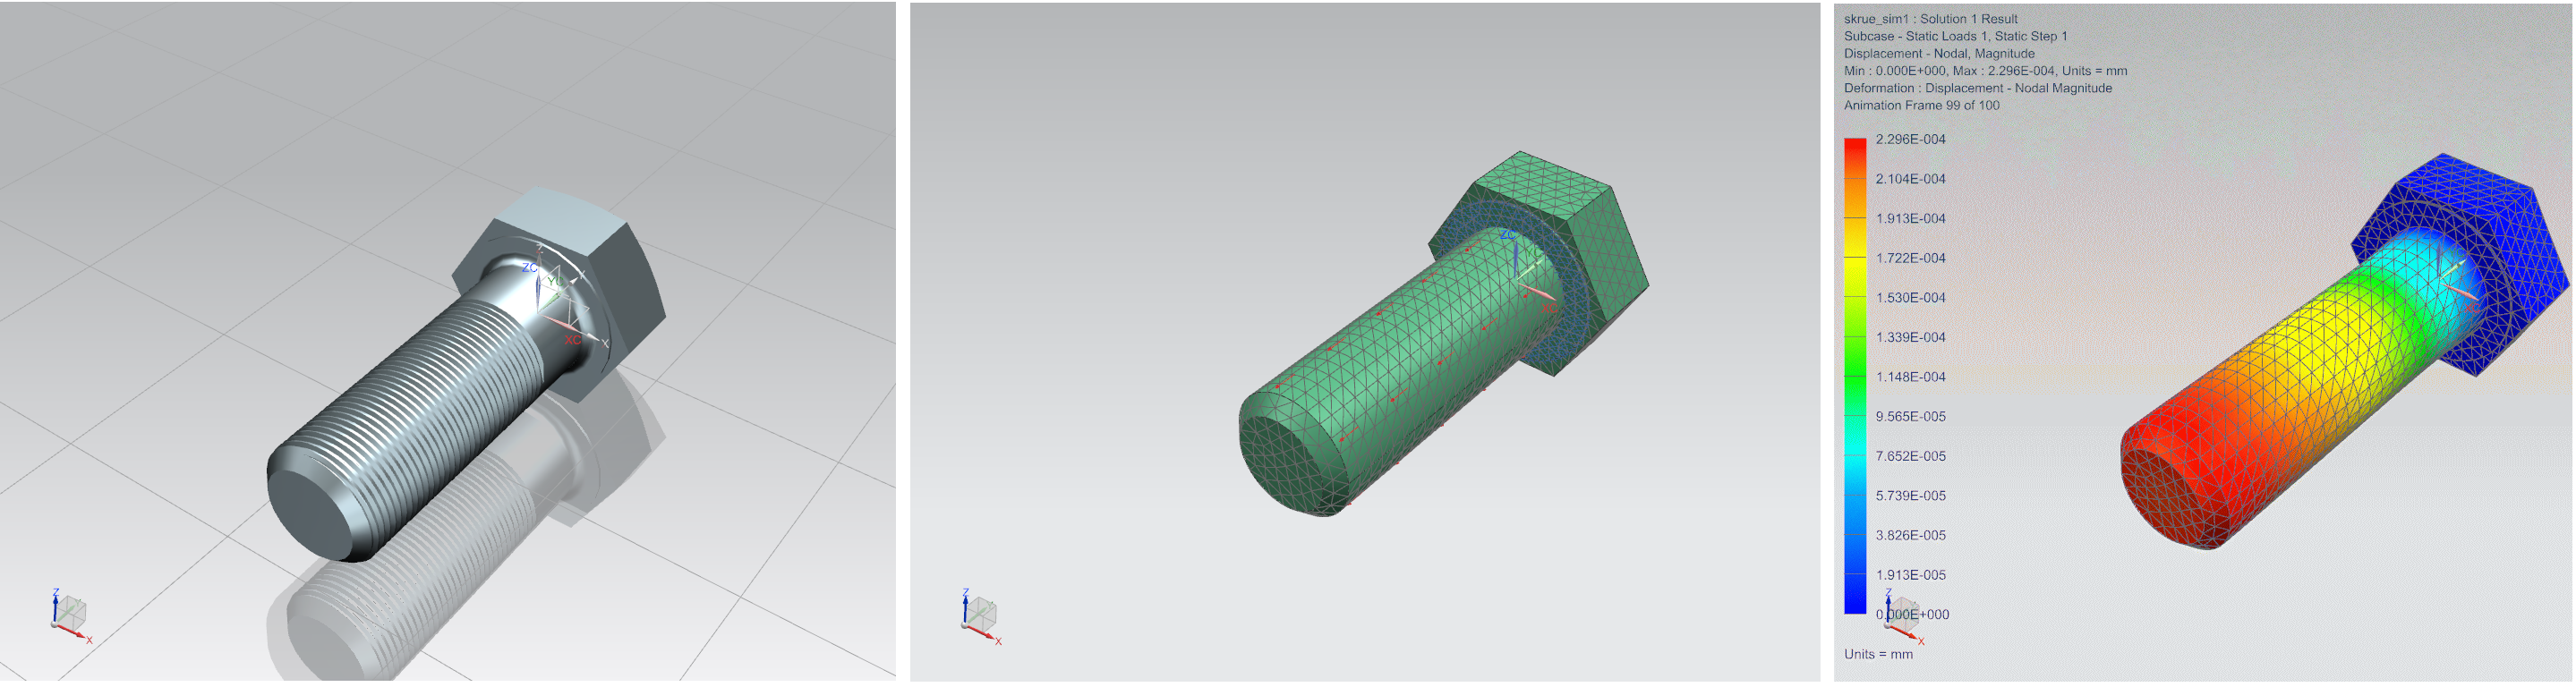
\includegraphics[width=1.00\textwidth]{images/Rapportbilde_skrue.png}
		\label{fig:FEMskrue}
		\caption{FEM-analyse av belastninger på tiltrukket bolt. Fra venstre til høyre: Modellert bolt, Forenklet og tilført mesh, Styrkeberegninger (her illustrert ved deformasjon}
	\end{figure}
\begin{figure}[H]
		\centering
		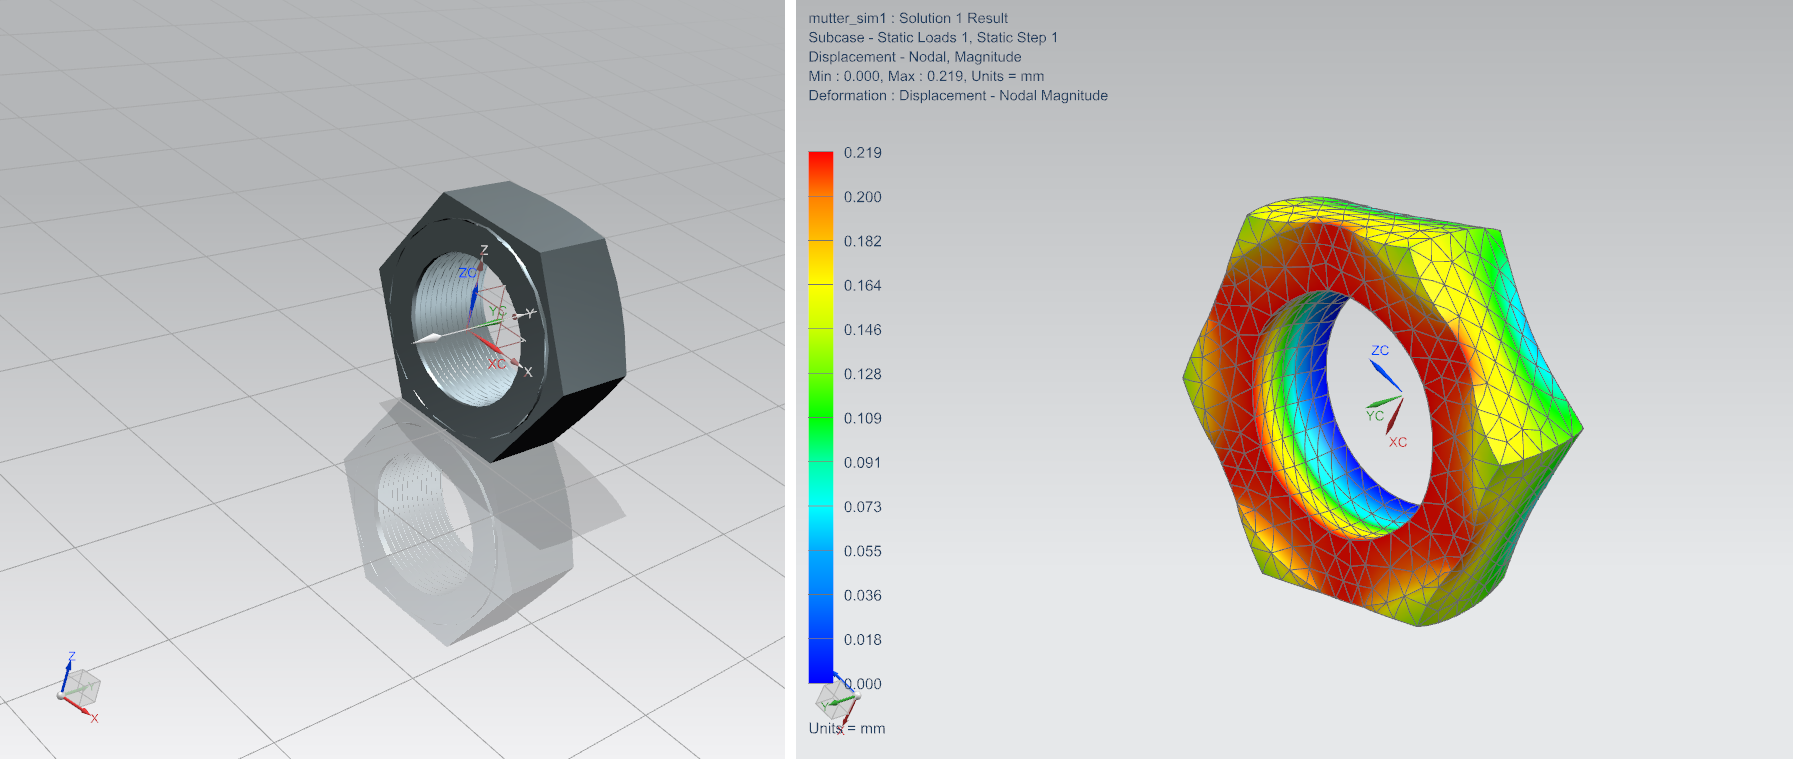
\includegraphics[width=1.00\textwidth]{images/Rapportbilde_mutter.png}
		\label{fig:FEMmutter}
		\caption{FEM-analyse av belastninger på tiltrukket mutter. Fra venstre til høyre: Modellert mutter, Styrkeberegninger her illustrert ved deformasjon.}
	\end{figure}

 
	%\input{section/hardware}
	%%TODO: Formatering
\section{Software}
All sensordata mottas fra microcontrollerene hos en sentral enhet som skal ta seg 
av analyse og visualisering av dataene. Hvordan analysen og visualiseringen av 
dataene skal fungere avhenger av hvilken type sensorer som brukes i systemet. I 
denne rapporten taes det for seg tre forskjellige typer sensorer, strekklapp, 
trykksensor, og vibrasjonssensor. På grunn av likheter i verdier og analysering 
av verdier velger vi å omtale strekklappsensor og trykksensor sammen som 
boltsensor.

\subsection{Analyse av data}
Hvordan data skal analyseres vil være avhengig av hvilken type sensor man velger 
for systemet. 

\subsubsection{Boltsensor}
Ved bruk av enten strekklapp eller trykksensor vil man få inn en verdi per bolt 
om hvor mye en bolt er strammet til. Analysen vil gå ut på å sammenligne målinger 
med grenseverdier som er satt for de ulike sensorene.

{\bf Utfordringer}\\
Utfordringer ved bruk av strekklapp/trykksensor %TODO

\subsubsection{Vibrasjonssensor}
Ved bruk av vibrasjonssensor vil man få inn verdier fra en sensor som lytter på 
akslingene. Dersom man bruker av en sensor per aksling vil man kunne detektere at 
det er en feil på et av hjulene på akslingen. Ved bruk av to sensorer per aksling 
vil man kunne se hvilket hjul problemet gjelder. Dette kan gjøres ved å se 
hvilken sensor som sendte lyden først.

En kjent feil (feks. løse hjulbolter) vil høre til et kjent frekvensområde, som 
kan brukes til å skille ut eventuelle feil som skulle oppstå.

{\bf Utfordringer}\\
Dersom man kjører på annet underlag slik som snø eller grus, vil dette kunne 
skape problemer med vibrasjonssensor. Frekvensene som mottas fra sensorene vil 
variere etter hvilket underlag man kjører på. Det vil si at frekvensområder for 
kjente feil også bør tilpasses etter underlaget. Dette kan i teorien løses ved å 
enten lagre kjente frekvenseområder for forskjellige underlag. Eventuelt kan man 
sammenligne hver sensor med nåværende gjennomsnitt for alle sensorene for å 
skille ut mulige feil. 

På grunn av uregelmessigheter i veibanen slik som et hull i veien eller flaske 
man kjører på, vil det være nødvendig å klassifisere noe som et problem dersom 
frekvensen som skiller seg ut er gjeldene i mer enn en gitt tid.

\subsection{Visualisering}
Dataene som mottas skal visualiseres etter å ha blitt analysert for å varsle 
sjåfør ved eventuelle problemer. Når det oppstår et problem skal sjåføren bli 
varslet i form av en visuell varsling på et display.

\subsubsection{Strekklapp/Trykksensor}
Sjåføren vil til en hver tid ha mulighet for å se verdiene for de ulike dekkene 
og sensorene. 

Ved bruk av farger kan man visualisere hvor løse mutterne på et hjul er, samt se 
verdier for hver sensor om ønskelig. Dersom man får inn en verdi fra 
strekklappsensor eller trykksensor som er høyere enn en grenseverdien for løse 
muttere, vil man få opp en advarsel på skjermen. Varselen vil variere fra en 
mindre notifikasjon i hjørnet av skjermen for mindre alvorlige feil, til en 
større varsel midt på skjermen for mer alvorlige feil.

{\bf Utfordringer}\\
En utfordring ved bruk av strekklapp eller trykksensor vil kunne ligge i den 
visuelle representasjonen av feilmeldingen. Det kan i utgangspunktet virke som 
en god idé å vise detaljer ned til hvilken bolt det er registrert avvik i. Det 
som da blir problemet er å vise hvilken posisjon hjulet har rotasjonsmessig for 
å la fører slippe å ettertrekke alle mutre på gitte hjul.

\subsubsection{Vibrasjonssensor}
Visualisering ved bruk av vibrasjonssensorer vil først og fremst være varsling 
ved eventuelle feil som måtte oppstå. Ut i fra om man velger å ha en eller to 
sensorer per aksling vil man få informasjon om hvilket hjul eller aksling 
problemet gjelder. Her vil man også få opp en liten notifikasjon ved mindre 
alvorlige feil og et større varsel ved mer alvorlige feil . Ved å trykke seg 
inn på varselen eller notifikasjonen vil man kunne få en bedre oversikt over 
problemene. Symboler og farger vil vise til hvilke feil som er gjeldene og hvor 
alvorlig det er.

{\bf Utfordringer}\\
%TODO
%\input{section/Markedsundersøkelse}
	%generelt
	%4 p'er
\section{Løsning}
	%\input{section/løsning}
	%\input{section/hardwareløsning}
	%\input{section/softwareløsning}
	%\input{section/løsningdiskusjon}
%\input{section/Konklusjon}
%\input{section/Referanseliste}
%\input{section/Vedlegg}
%%%
% End includes
%%%
\addcontentsline{toc}{chapter}{Bibliography}
\bibliographystyle{plain}
\thispagestyle{plain}

\begin{thebibliography}{10} %Foreløpig: oppdater dette nr som man legger til item
	
	\bibitem{tdt4856}{
		\emph{ntnu.no}
		N.P.. Web. Mar 04 2015
		<\url{http://www.ntnu.no/eit/tdt4856}>
	}
	
	\bibitem{hjulmist}{
		\emph{egenbil.no}
		N.P.. Web. Mar 04 2015
		<\url{ http://www.egenbil.no/nyttig-aa-vite/hjulmist}>
	}
		
	\bibitem{NL-skive}{
		\emph{nord-lock.com}
		N.P.. Web. Mar 04 2015
		<\url{http://www.nord-lock.com/nord-lock/wedge-locking/washers/introduction/}>
	}
	
	\bibitem{NL-hjulbolt}{
		\emph{nord-lock.com}
		N.P.. Web. Mar 04 2015
		<\url{	http://www.nord-lock.com/nord-lock/wedge-locking/wheel-nut/introduction/}>
	}
	
	\bibitem{checkpoint1}{
		\emph{cpsafety.com.au/}
		N.P.. Web. Mar 04 2015
		<\url{http://www.cpsafety.com.au/product-checkpoint.php}>
	}
		
	\bibitem{dekkslitasje-GT6}{
		\emph{pro-gmedia.com}
		N.P.. Web. Mar 04 2015
		<\url{http://s.pro-gmedia.com/videogamer/media/images/ps3/gran_turismo_6/screens/gran_turismo_6_220.jpg}>
	}

	\bibitem{FriksjonsfaktorGjenger}{
		\emph{kamax.com}
		N.P.. Web. Feb 25 2015
		<\url{http://www.kamax.com/fileadmin/user_upload/dokumente/pdf/Bolt_and_Screw_Compendium.pdf}>
	}

	\bibitem{FEManalyse}{
		Bell, Kolbein. \emph{An engineering approach to FINITE ELEMENT ANALYSIS of linear structural mechanics problems}. 1st ed. Akademika forlag, 2013. Print.
	}
	
	\bibitem{asme}{
		\emph{asme.org}
		N.P.. Web Apr 28 2015
		<\url{http://vibrationacoustics.asmedigitalcollection.asme.org/article.aspx?articleID=1840144}>
	}

	\bibitem{sagepub}{
		\emph{sagepub.com}
		N.P.. Web Apr 28 2015
		<\url{http://shm.sagepub.com/content/7/4/309.full.pdf}>
	}

	\bibitem{canbus}{
		\emph{hellanor.no}
		N.P.. Web. Mar 25 2015
		<\url{http://www.hellanor.no/filestore/PDF_filer/Teknisk_informasjon/Hella/Elektronikk/can_bus.pdf}>
	}
	
	\bibitem{adc}{
		\emph{analog.com}
		N.P.. Web. Apr 22 2015
		<\url{http://www.analog.com/en/products/analog-to-digital-converters.html}>
	}
	
	\bibitem{dsp}{
		\emph{dspguide.com}
		N.P.. Web. Apr 22 2015
		<\url{http://www.dspguide.com/ch28.htm}>
	}

	\bibitem{wheatstone}{
		\emph{electronics-tutorials.ws}
		N.P.. Web. Mar 25 2015
		<\url{http://www.electronics-tutorials.ws/blog/wheatstone-bridge.html}>
	}

	\bibitem{nyquist}{
		\emph{lavryengineering.com}
		N.P.. Web. Mar 18 2015
		<\url{http://web.archive.org/web/20060614125302/http://www.lavryengineering.com/documents/Sampling_Theory.pdf}>
	}
	
	\bibitem{PCBmail}{
		Erik Nordby \emph{Semitronic AS}.
		Personal Communications Mar 25 2015
	}
	
	\bibitem{innovasjonnorge}{
		\emph{www.innovasjonnorge.no}
		N.P.. Web. May 1 2015
		<\url{http://www.innovasjonnorge.no/no/finansiering/etablerertilskudd/#.VUPiU2Ttmkp}>
	}
	
	\bibitem{skattefunn}{
		\emph{www.forskningsradet.no}
		N.P.. Web. May 1 2015
		<\url{http://www.forskningsradet.no/prognett-skattefunn/Artikkel/Hvem_kan_fa_stotte__og_hvor_mye/1253987672197}>
	}

	\bibitem{lastebilprod-DAF}{
		\emph{daf.com/en}
		N.P.. Web. Mar 25 2015
		<\url{http://www.daf.com/en/about-daf/daf-trucks-nv/facts-and-figures}>
	}
	\bibitem{daimler}{
		\emph{daimler.com}
		N.P.. Web. Mar 25 2015
		<\url{https://www.daimler.com/company/business-units/daimler-trucks}>
	}
	
	\bibitem{MVC}{
		\emph{apple.com}
		N.P.. Web. Apr 20 2015
		<\url{https://developer.apple.com/library/mac/documentation/General/Conceptual/DevPedia-CocoaCore/MVC.html}>
	}
	
	\bibitem{firmware}{
		\emph{liteonit.eu}
		N.P.. Web. Apr 22 2015
		<\url{http://www.liteonit.eu/what_is_firmware.html}> 
	}
	
	\bibitem{embedded}{
		\emph{ece.ncsu.edu}
		N.P.. Web. Apr 20 2015
		<\url{http://www.ece.ncsu.edu/research/cas/ecs}> 
	}
	
	\bibitem{altium}{
		\emph{altium.com}
		N.P.. Web. Apr 27 2015
		<\url{http://www.altium.com/}> 
	}
	
	\bibitem{Fourier}{
		\emph{gsu.edu}
		N.P.. Web. Apr 20 2015
		<\url{http://hyperphysics.phy-astr.gsu.edu/hbase/audio/fourier.html}> 
	}

	\bibitem{aamodt94}{
		Aamodt, Agnar og Plaza, Enric. \emph{Case-Based Reasoning: Foundational Issues, Methodological Variations, and System Approaches.}
		AI Communications, Vol. 7 Nr. 1, March 1994, pp 39-59.
	}
	
\end{thebibliography}	
\end{document}